\section{UI Design}
\label{research:UIDesign}
I wanted to research a variety of UI design styles used in the industry to find inspiration for my own design. I looked at different types of user interfaces, including those used in mobile applications, web applications, and desktop software.

\subsection*{Glass Morhphism}
\begin{figure}[h]
    \centering
    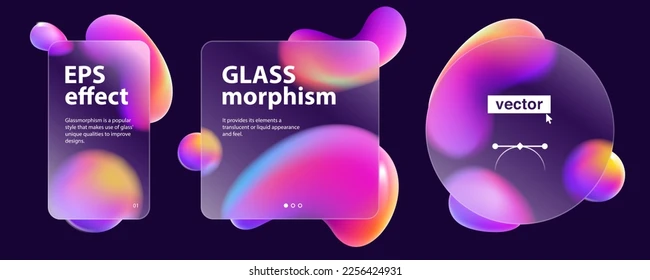
\includegraphics[width=0.6\textwidth]{Research/6_UIDesign/media/Glassmorhpism.png}
    \caption{Example of Glassmorphism UI Design}
    \label{fig:glassmorphism}
\end{figure}
Glass morphism is perhaps my favourite of the current design trends implemented by a variety of products. It plays with colour, blur and light reflections. This design looks stunning when used well but has a number of downsides that often don’t make it practical for use cases that have a large number of Ui elements. Firstly it is very performance heavy which results in complex designs slowing down systems, secondly without having bold colour as a tool to show importance it be can be complex to show a user which tools are move crucial to their use case.


\subsection*{Newmorphism }
\begin{figure}[h]
    \centering
    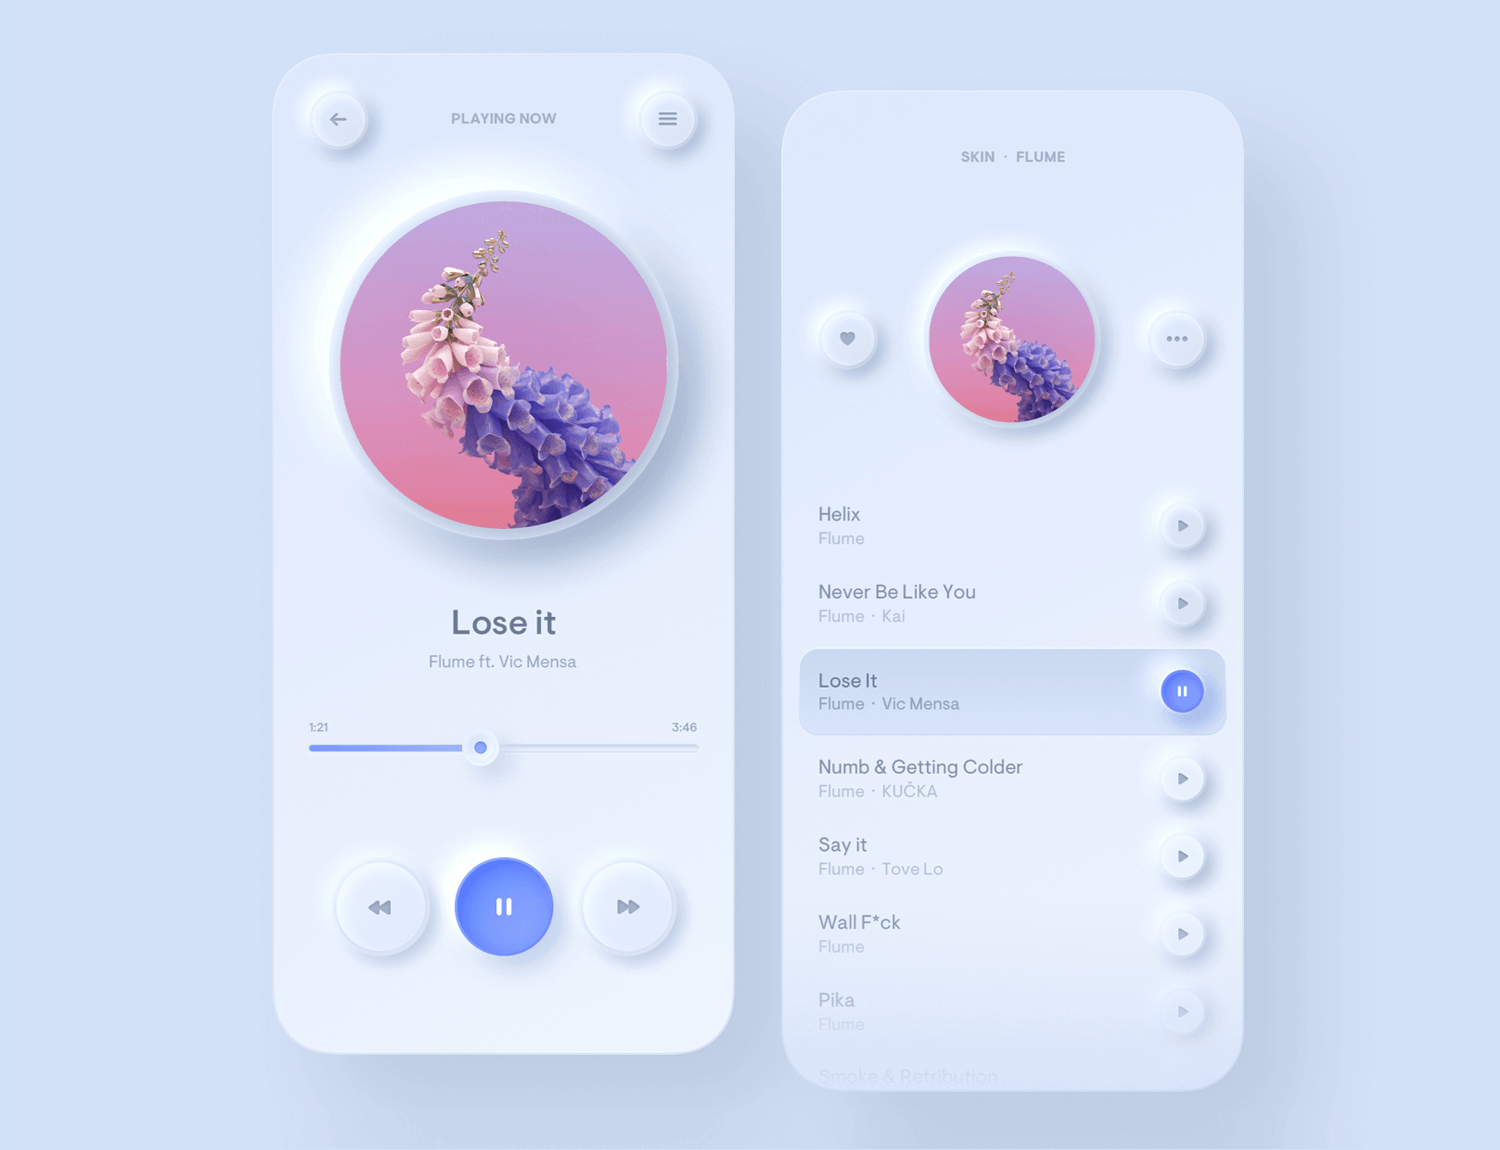
\includegraphics[width=0.6\textwidth]{Research/6_UIDesign/media/Newmorphism.png}
    \caption{Example of Newmorphism UI Design}
    \label{fig:newmorphism}
\end{figure}

This design style really appeals to me as being smooth, slick and very easy on the eye. Information is portrayed using depth on a virtual canvas, replacing 'louder' user messaging with more subtle stylistic representations of detail. While this latter point is the foundation of my liking for the style, it also has some concerns regarding accessibility to those with reduced vision and even is less intuitive to a user perhaps not well versed in software design meaning. Subtle shade differences highlighting critical detail will probably not coexist with my goal of software being easy to access for all


\subsection*{claymorhpism}
\begin{figure}[h]
    \centering
    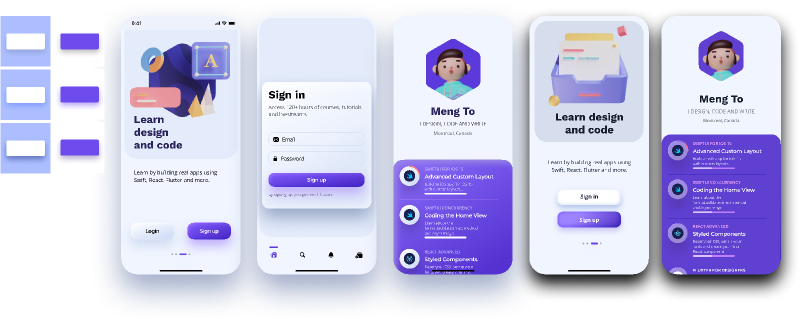
\includegraphics[width=0.6\textwidth]{Research/6_UIDesign/media/Claymorhpism.png}
    \caption{Example of Claymorphism UI Design}
    \label{fig:claymorphism}
\end{figure}
Clay morphism takes inspiration from neomorphism but replaces subtler shadows with much more vivid colour usually within a duotone design. This is much easier to understand but can have limitations within larger interfaces as menus can be hard to differentiate in importance

\subsection*{Skewmorhpism}
\begin{figure}[H]
    \centering
    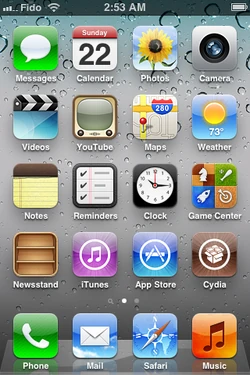
\includegraphics[width=0.2\textwidth]{Research/6_UIDesign/media/Skewmorphism.png}
    \caption{Example of Skewmorphism UI Design}
    \label{fig:skewmorphism}
\end{figure}
Skew morphism is an excellent design philosophy for making software approachable for those who aren't as familiar to technology. It uses detailed 2.5/3d objects from real life to represent the functions of interface elements. Whilst this is highly informative I personally don’t lie this style primarily due to the visual overload it can create; it can be hard to find different options which results in little speed gain from an experienced user vs a novice which does have its pros and cons but it mainly negative for those wanting to use the software daily

\subsection*{Neubrutalism}
\begin{figure}[H]
    \centering
    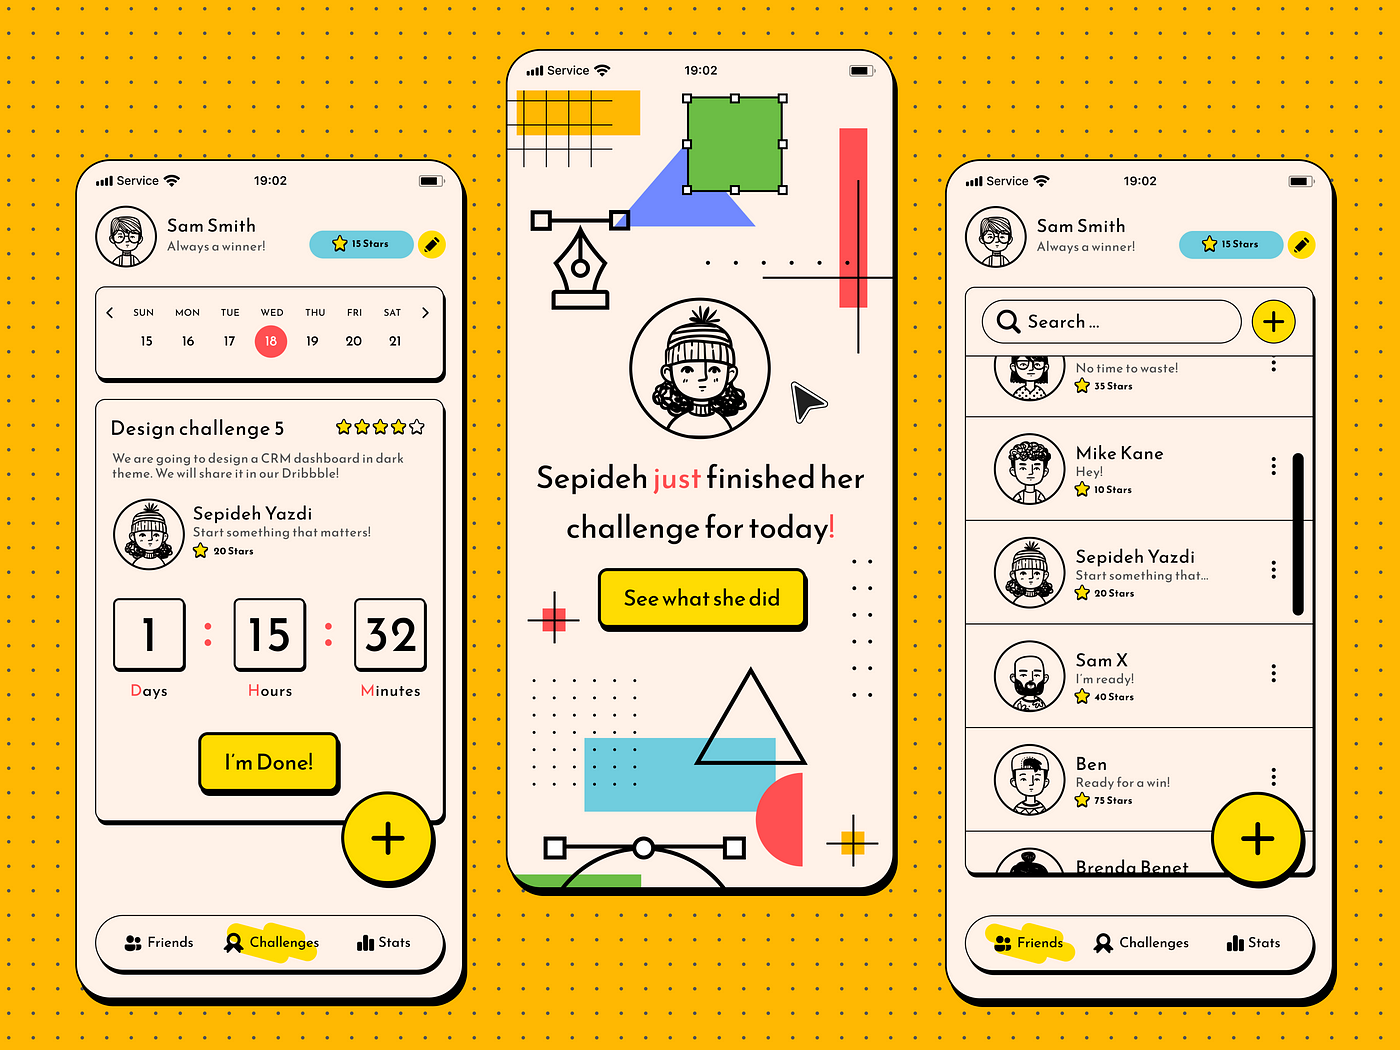
\includegraphics[width=0.2\textwidth]{Research/6_UIDesign/media/Neubrutalism.png}
    \caption{Example of Neubrutalism UI Design}
    \label{fig:neubrutalism}
\end{figure}
Brutalist UI designs make no effort to replicate real life with their representation of icons and instead use bold shapes and bright tones to highlight visual importance to the user. While I personally am not a huge fan of the design style I can appreciate its merits in accessibility to those with limited visual sight. The design however can be confusing for those not as technically versed to use due to the lack of links it makes to the world around us

\subsection*{Flat design}
\begin{figure}[H]
    \centering
    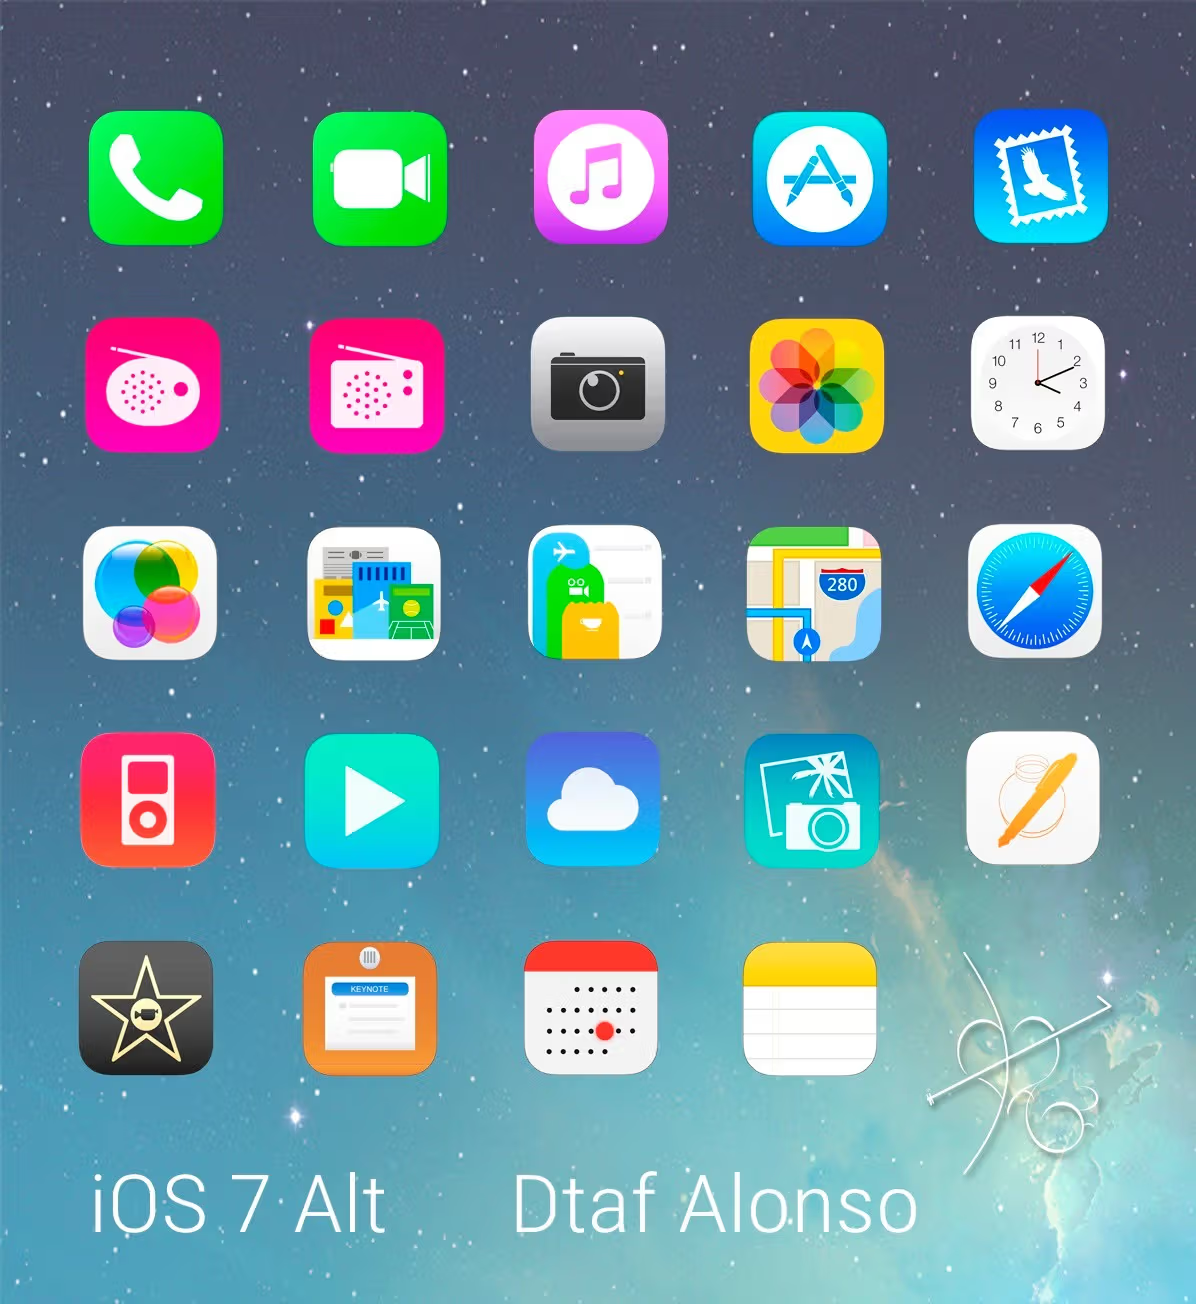
\includegraphics[width=0.2\textwidth]{Research/6_UIDesign/media/FlatDesign.png}
    \caption{Example of Flat Design UI}
    \label{fig:flatdesign}
\end{figure}
Similar to Skew morphism in that digital concepts are represented by icons harking back to real life, Flat designs implies these ideas down into flat, unified symbols formed by primitive shapes and typography. In my opinion this proves a nice balance between the ease of fully world representative icons, and the (often hard to interpret) digital icons which adorn most websites. Flat design looks best when combined with other techniques which inform colour, shadow and vibrancy effects to help create a unified visual style

